% This is a LaTeX template
% for preparing documents for ITTMM conference

\documentclass[60x84/16,8pt]{ittmm}

% Убедительная просьба к авторам не редактировать файл definition.tex
\usepackage[T1,T2A]{fontenc}
\usepackage{ucs}
\usepackage[utf8x]{inputenc}
\usepackage[english,russian]{babel}

%% Расширенная математика

\usepackage{amsmath}
\usepackage{amssymb}
\usepackage{amscd}

\usepackage{mathtools}
\usepackage{listings}
\mathtoolsset{
showonlyrefs=true,
mathic=true,
}

\allowdisplaybreaks

%% Работа с графикой

\usepackage{graphicx}

%% hyperref

\usepackage{hyperref}
\hypersetup{backref,
 colorlinks=false}
\hypersetup{pdfborder=0 0 0}

%% local definitions

\geometry{twoside}
\geometry{bindingoffset=0pt}

\geometry{includehead}
\geometry{hmargin={16mm,16mm},vmargin={12mm,13mm}}
\geometry{marginparwidth=0pt,marginparsep=0pt}
\geometry{headheight=0pt}
\geometry{headsep=\baselineskip}

\pagestyle{empty}

\usepackage{cite}

\makeatletter
\g@addto@macro\@maketitle@hook@post{%
 \iflanguage{english}{%
   \bibliographystyle{elsarticle-num}
 }{%
   \bibliographystyle{ugost2008l}
 }
}
\makeatother

%%% Local Variables:
%%% mode: latex
%%% coding: utf-8-unix
%%% End:


\begin{document}

% Укажите индекс УДК, соответствующий Вашей работе.
\udc{004.94}

\title{Автоматизация процессов моделирования и измерения сетевых характеристик в Mininet}

\author{С. М. Наливайко}

\address{Кафедра прикладной информатики и теории вероятностей\\
  Российский университет дружбы народов\\
  ул. Миклухо-Маклая, д.6, Москва, 117198, Россия}

\email{\url{1032183644@rudn.ru}}

\begin{abstract}
  Среда виртуального моделирования Mininet позволяет использовать
  реальные сетевые приложения, сетевые протоколы и ядро Unix/Linux для
  тестирования и анализа характеристик моделируемых в ней компьютерных
  сетей и сетевых протоколов. Процесс моделирования в Mininet,
  указание на используемые при моделировании протоколы, задание
  параметров сети и протоколов и т.\,п. проводится с помощью команд
  терминала. Это достаточно рутинный процесс. В данной работе
  предложено описание разработанной программы для автоматизации как
  процесса задания параметров моделируемой сети, так и процесса
  обработки полученных результатов. Программа представляет собой набор
  модулей на языке программирования Python, причем каждый из модулей
  отвечает за свой круг задач, будь то модуль для отрисовки графиков
  или модуль проведения замеров на интерфейсе. Каждый из модулей
  самодостаточен и может быть использован отдельно.
\end{abstract}

\keywords{информационные технологии, моделирование сетей, Mininet,
  автоматизация, измерение сетевых характеристик}


% \thanks{Рукопись должна содержать УДК, который рекомендуется брать из
%   следующего источника: \url{http://www.mathnet.ru/udc.pdf}.}

\alttitle{Automation of Mininet modeling and network performance
  measurement processes}

\altauthor{S. M. Nalyvaiko}

\altaddress{Department of Applied Probability and Informatics\\
Peoples' Friendship University of Russia\\
Miklukho-Maklaya St., 6, Moscow, 117198, Russian Federation}


\begin{altabstract}
  The Mininet virtual simulation environment allows to use some real
  network applications, network protocols, and the Unix/Linux kernel
  to test and analyze characteristics of computer networks and network
  protocols modeled in it. The modeling process in Mininet, indication
  of the protocols used in the simulation, setting network and
  protocol parameters, etc., is carried out by using terminal
  commands. It’s a routine process.  In this paper, the description of
  the program for automating both the process of setting the
  parameters of the simulated network and the process of processing
  the obtained results is proposed.  The program is the set of modules
  in the Python programming language, and each of the modules is
  responsible for its own range of tasks, whether it is a module for
  drawing graphs or a module for taking measurements on the
  interface. Each of the modules is self-sufficient and can be used
  separately.
\end{altabstract}

\altkeywords{information technology, network modeling, Mininet,
  automation, performance measurement}

\maketitle

\section{Введение}
\label{sec:intro}

Создание сети не может обходиться без предварительного анализа и
прототипирования. Для таких задач могут использоваться современные
программы, которые позволяют создавать и испытывать сети без реальных
сетевых компонентов. Такое решение дешево в построении, а сбор данных
сетевых характеристик заметно ускоряется и упрощается. Есть несколько
программных средств для моделирования сети, например gns3~\cite{gns3},
ns-3~\cite{ns3}, Cisco Packet Tracer~\cite{cpt} и др. Для измерения
характеристик сети используются другие средства, например,
Wireshark~\cite{wireshark}, Total Network Monitor~2~\cite{tnm2},
Zabbix \cite{zabbix} и др. Выбрав средство моделирования для
подготовки испытательного стенда и средство мониторинга сетевых
характеристик можно приступать к анализу и прототипированию сети с
заданными параметрами.  Настройка сетевых компонентов вручную в среде
симуляции представляет собой достаточно рутинный процесс.

Целью данной работы является построение средства автоматизации
процессов моделирования и измерения сетевых характеристик передачи
данных. В качестве среды моделирования была выбрана программа
Mininet~\cite{mininet}, так как она позволяет использовать реальные
сетевые приложения, сетевые протоколы и ядро Unix/Linux для
тестирования и анализа характеристик моделируемых в ней компьютерных
сетей и сетевых протоколов, а в качестве программ, которые позволяют
измерять сетевые характеристики, были выбраны iproute2~\cite{iproute2}
и iperf3~\cite{iperf3}.

\section{Решение задачи автоматизации построения виртуальной сети и измерения сетевых характеристик} 
\label{sec:base-section}

\subsection{Недостаток процесса построения сети и ее тестирования}

Mininet предоставляет исчерпывающий API~\cite{mininet-api} для
создания виртуальной сети. API предоставлен для языка программирования
Python, поэтому, чтобы приступить к работе, требуется с помощью
программы pip установить пакет mininet. Установив библиотеку, ее можно
импортировать в рабочий файл.

Сначала требуется создать топологию сети. Пример простой топологии,
состоящей из двух хостов h1 и h2, а также соединяющих их двух
коммутаторов s1 и s2, представлен на рис.~\ref{fig:example_topo}.

%![Пример топологии](img/example_topo.png)
\begin{figure}[!h]
        \centering
        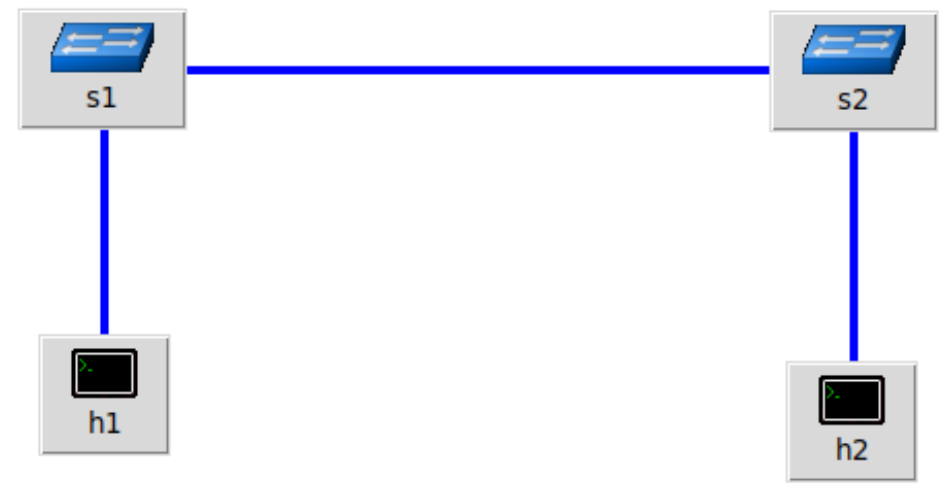
\includegraphics[width=0.5\linewidth]{example_topo2}
        \caption{Пример топологии}
        \label{fig:example_topo}
\end{figure}

Предполагается, что в данной сети будут действовать следующие правила:
\begin{itemize}
\item скорость передачи данных ограничена;
\item максимальная пропускная способность соединения h1-s1 равна 100
  Мбит/с;
\item максимальная пропускная способность соединения s2-h2 равна 50
  Мбит/с;
\item на коммутаторе s2 стоит дисциплина обработки очередей FIFO с
  максимальным количеством пакетов, равным 30;
\item потери в сети составляют 0.001\%;
\item задержка имеет нормальное распределение с математическим
  ожиданием в 30~мс и с дисперсией в 7~мс.
\item в сети работает алгоритм для работы с перегрузками TCP Reno.
\end{itemize}

Тогда процесс создания и использования сети с данной топологией с
помощью Python и Mininet-API будет иметь несколько этапов:
\begin{itemize}
\item описание класса топологии в файле;
\item создание сети с помощью описанной топологии;
\item старт сети;
\item настройка сетевых компонентов из терминала;
\item тестирование  сети;
\item остановка работы сети.
\end{itemize}

Предположим, что нам потребовалось поменять количество узлов,
коммутаторов, сетевые характеристики или еще что-либо. Нам потребуется
снова править код? Да, однако, можно автоматизировать данный процесс.


\subsection{Автоматизация процесса создания сети}

Метод автоматизации основан на создании конфигурационного
toml-файла~\cite{toml}, из которого программа на языке
программирования Python будет считывать данные и собственно учитывать
изменения при настройке параметров топологии, мониторинговых
характеристик.

Приведём пример  toml-файла (см. листинг~\ref{lst1}).
%Тогда, настройки в toml-файле будут иметь следующий вид:

\begin{lstlisting}[breaklines=true, numbers=left,
  basicstyle=\ttfamily\small, xleftmargin=\parindent, caption={Пример  toml-файла с
    описанием топологии и настроек сети}, label=lst1] 
# device settings
[devices]

[devices.h1]
name = "h1"
ip = "10.0.0.1"
cmd = [
"sysctl -w net.ipv4.tcp_congestion_control=reno"
]

[devices.h2]
name = "h2"
ip = "10.0.0.2"
cmd = [
"sysctl -w net.ipv4.tcp_congestion_control=reno"
]

# switch settings
[switches]

[switches.s1]
name = "s1"
[switches.s2]
name = "s2"

# link settings
[links]

pairs = [
["h1", "s1"],
["s1", "s2"],
["s2", "h2"]
]

cmd = [
"tc qdisc replace dev s1-eth2 root handle 10: tbf rate 100mbit burst 50000 limit 150000",
"tc qdisc add dev s1-eth2 parent 10: handle 20: netem loss 0.001% delay 30ms 7ms distribution normal",
"tc qdisc replace dev s1-eth1 root handle 10: tbf rate 100mbit burst 50000 limit 150000",
"tc qdisc add dev s1-eth1 parent 10: handle 20: netem loss 0.001% delay 30ms 7ms distribution normal",
"tc qdisc replace dev s2-eth2 root handle 10: tbf rate 50mbit burst 25000 limit 75000",
"tc qdisc add dev s2-eth2 parent 10: handle 15: pfifo limit 30",
"tc qdisc replace dev s2-eth1 root handle 10: tbf rate 50mbit burst 25000 limit 75000"
]
\end{lstlisting}

В представленном toml-файле раздел \textbf{devices} отвечает за
настройку конечных узлов сети, раздел \textbf{switches}~--- за
настройку коммутаторов, а раздел \textbf{links}~--- за настройку
соединений узлов сети и конфигурацию интерфейсов коммутаторов.

На хостах указывается ip-адрес, имя хоста и алгоритм работы с
перегрузками. На коммутаторах прописывается только имя, однако, список
настроек можно расширить, изменив программную логику в классе с
топологией. В разделе \textbf{links} явно указывается, какие пары
сетевых устройств соединяются, и команды, которые настраивают
дисциплину очередей на интерфейсах. Подробнее о дисциплинах очередей
можно прочесть в~\cite{qdisc}.

Имея подобный конфигурационный toml-файл, его можно прочесть с помощью
средств Python, обработать и положить требуемые значения в объекты.
Такой подход позволяет строить сколь угодно большие топологии без
правки логики приложения.

\subsection{Автоматизация процесса мониторинга}

Вернемся к toml-файлу и добавим параметры для класса мониторинга
(см. листинг~\ref{lst2}).

\begin{lstlisting}[breaklines=true, numbers=left,
  basicstyle=\ttfamily\small, xleftmargin=\parindent, caption={Пример  toml-файла с
    описанием мониторинга сетевых характеристик}, label=lst2]
[monitoring]
monitoring_time = 30
monitoring_interval = 0.1
host_client = "h1"
host_server = "h2"
interface = "s2-eth2"
iperf_file_name = "iperf.json"
iperf_flags = ""
queue_data_file_name = "qlen.data"
plots_dir = "plots_dir"
plots_format = "pdf"
\end{lstlisting}


В представленном коде указаны все параметры, которые могут
понадобиться для задачи анализа характеристик сети:
\begin{itemize}
\item monitoring\_time~--- время мониторинга сети;
\item monitoring\_interval~--- интервалы между замерами длины очереди;
\item host\_client~--- узел, который будет отправлять данные;
\item host\_server~--- узел, который будет принимать данные;
\item interface~--- интерфейс, на котором будет мониторится размер
  очереди;
\item iperf\_file\_name~--- имя файла с отчетом мониторинга iperf;
\item iperf\_flags~--- iperf-флаги клиента;
\item queue\_data\_file\_name~--- имя файла с отчетом мониторинга длины
  очереди;
\item plots\_dir -- директория со всеми графиками сетевых
  характеристик.
\end{itemize}


Мониторинг запускается после старта сети, а так как у нас
отслеживаются как сетевые характеристики (пропускная способность,
задержки, повторная отправка пакетов и т.\,д.), так и размер длины
очереди на интерфейсе коммутатора, то следует пустить 2 параллельных
потока под эти нужды. Эти и прочие детали реализации класса
мониторинга не рассмотрены в данной работе, однако, полный исходный
код можно найти по адресу
\href{https://github.com/nalivaykosergey/net_automatic_monitoring}{github.com/nalivaykosergey/net\_automatic\_monitoring}.


\subsection{Объединение автоматизированных модулей}

Имея готовый класс топологии и класс мониторинга, можно создать объекты
этих классов, запустить сеть, включить мониторинг сети, построить
графики и так далее. Диаграмма активностей для данного приложения
представлена на рис.~\ref{fig:monitoring}.

\begin{figure}[!h]
  \centering
  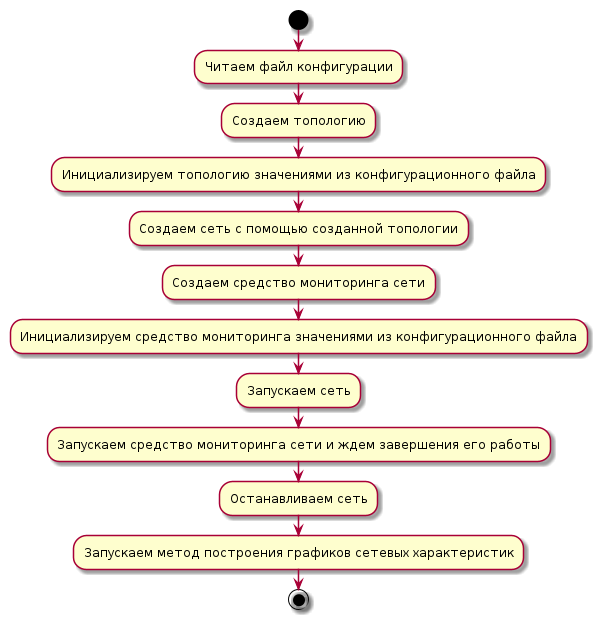
\includegraphics[width=0.7\linewidth]{monitoring}
  \caption{Диаграмма активностей для программы}
  \label{fig:monitoring}
\end{figure}


Диаграмма классов разработанного комплекса программ представлена на
рис.~\ref{fig:classdia}.

\begin{figure}[!h]
  \centering
  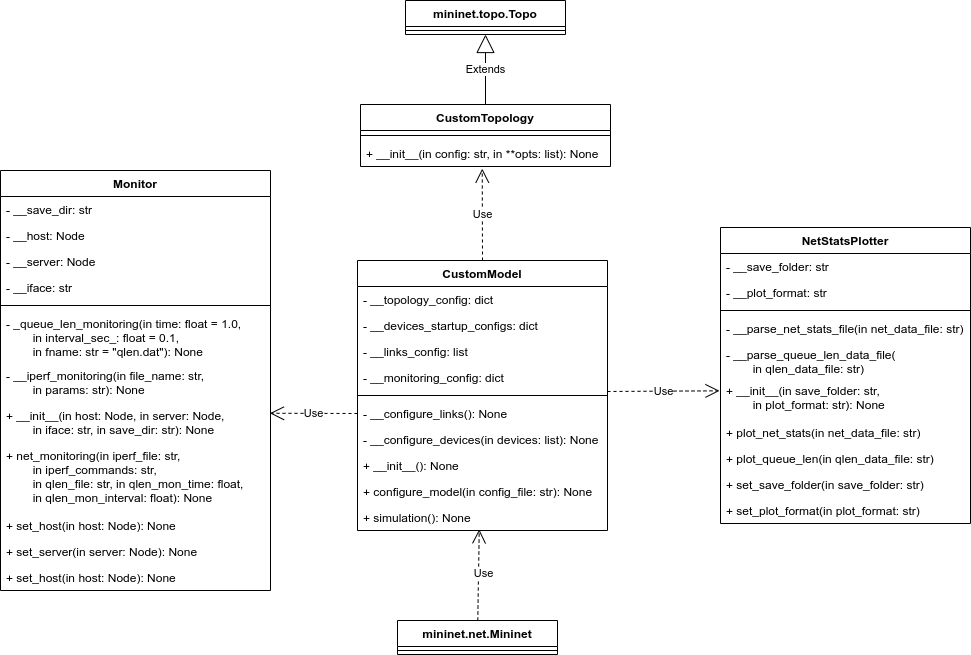
\includegraphics[width=1.0\linewidth]{classdia}
  \caption{Диаграмма классов приложения}
  \label{fig:classdia}
\end{figure}


% Теперь, зная принцип автоматизации, рассмотрим принцип взаимодействия
% с программой. Диаграмма классов представлена на
% рис.~\ref{fig:classdia}. 
Главным классом, включающим в себя все
остальные, является CustomModel. В методе \textbf{simulation}
создаются объекты классов Monitor, mininet.net.Mininet, Custom\-Topology
и NetStatsPlotter.

% Диаграмма активностей для данного метода
% представлена на рис.~\ref{fig:monitoring}.








Рассмотрим подробнее классы, создаваемые в методе \textbf{simulation}:
\begin{itemize}
\item mininet.net.Minet --- предоставляемый Mininet API класс,
  отвечающий за создание сети с топологией, указанной в
  CustomTopology;
\item CustomTopology --- класс топологии сети; % . Так как топология
  % задается автоматически, благодаря конфигурационному файлу, то и
  % править его каждый раз при изменении топологии сети не требуется.
\item Monitor --- класс, в котором происходят замеры сетевых
  характеристик исследуемой сети;
\item NetStatsPlotter --- класс, объект которого занимается
  построением графиков сетевых характеристик.
\end{itemize}

Точка входа в комплекс программ находится в файле \textbf{main.py}. Запустить
данный скрипт можно с помощью команды

\begin{lstlisting}[breaklines=true, basicstyle=\ttfamily\small, xleftmargin=\parindent]
  sudo ./main.py -c config/pfifo_config.toml
\end{lstlisting}

Параметр \textbf{-c} отвечает за местоположение конфигурационного файла.

Естественно, перед запуском скрипта требуется задать право на
исполнение файла. Делается это с помощью команды

\begin{lstlisting}[breaklines=true, basicstyle=\ttfamily\small, xleftmargin=\parindent]
  chmod +x main.py
\end{lstlisting}

После запуска в каталоге приложения появится директория с именем,
которое было указано в toml-файле. В ней содержатся графики изменения
сетевых характеристик и сырые данные, которые были обработаны объектом
класса NetStatsPlotter. Например, график изменение длины очереди на
интерфейсе s2-eth2 приведен на рис.~\ref{fig:qlen}. Видно, что
длина очереди не превышает размера 30 пакетов, что явно было указано в
настройках сети.


\begin{figure}[!h]
  \centering
  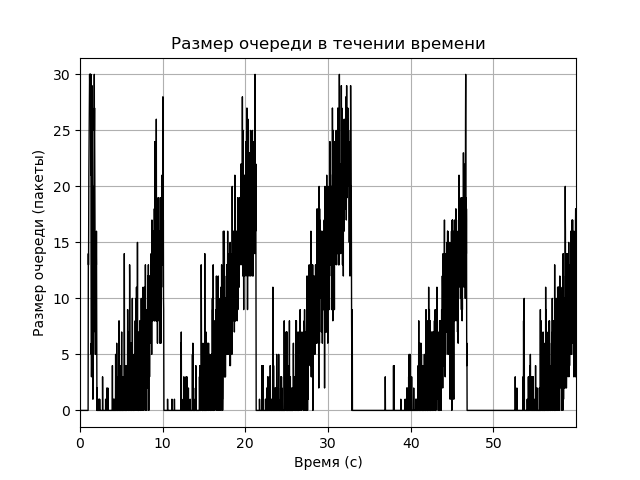
\includegraphics[width=0.75\linewidth]{qlen}
  \caption{График изменения длины очереди на интерфейсе s2-eth2}
  \label{fig:qlen}
\end{figure}

Процесс создания сети и мониторинга сетевых характеристик полностью
автоматизирован и не требует более вмешательств в программный код.


\section{Заключение}

Анализ работоспособности и производительности сети~--- неотъемлемая
часть работы сетевых инженеров. Современные программы, такие как
Mininet, предоставляют разработчикам быстрый и дешевый в построении
испытательный полигон, в котором можно проектировать и отлаживать
сетевые программы.

Решение по автоматизации, которое было предложено в ходе исследования,
ускоряет процесс перехода с создания сети на анализ ее
производительности. Имея несколько конфигурационных файлов, мы можем
быстро менять настройки сети и анализировать ее производительность
одной командой, не исправляя исходный код программы.


%% Возможно использовать bibtex.
\bibliographystyle{ugost2008l}
\bibliography{main}

\makealttitle

\end{document}
